\begin{center}
	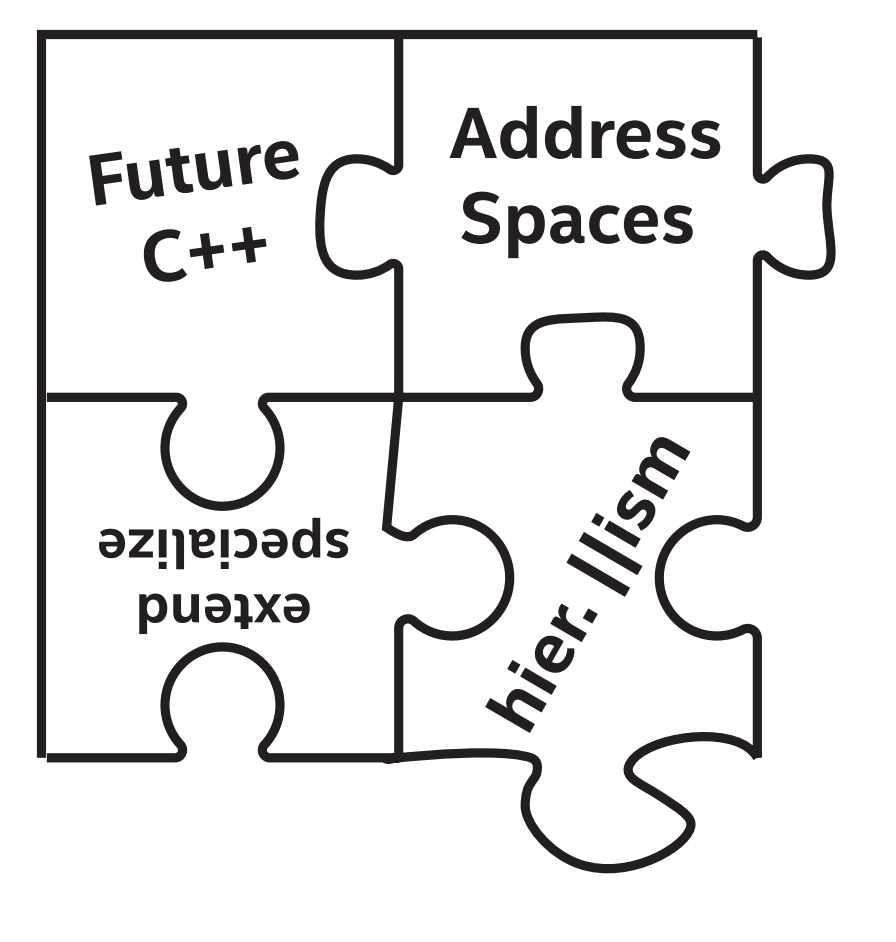
\includegraphics[width=0.3\textwidth]{content/chapter-20/images/1}
\end{center}

现在让我们感受一下平静,因为我们终于了解了使用SYCL和DPC++编程的所有知识。所有的谜团都已解开。\par

但还是要注意,这本书是在SYCL和DPC++刚出现的时候写的。随着第一个DPC++规范和SYCL 2020临时规范的发布,这是一个快速发展的时期,我们努力确保代码示例,与开源DPC++编译器编译的时候(2020年第三季)和执行广泛的硬件上时,出版了本书。但是,本结语中显示的未来代码到2020年年中还不能使用任何编译器进行编译。\par

结语中,我们对未来进行了展望。我们的水晶球可能有点难以解读。\par

这本书的绝大部分内容将会流传很长时间。也就是说,这是一个热门的区域,而且正在发生的变化可能会破坏我们已经了解的一些知识。这包括一些最初作为供应商扩展出现的项目,后来纳入了规范(比如子工作组和USM)。如此多的新特性将成为下一个SYCL标准的一部分,但这也使得讨论这些特性变得复杂:我们应该将这些特性称为供应商扩展、SYCL的实验/临时特性,还是SYCL的一部分?\par

这个结语提供了一个即将到来的DPC++特性的先睹所快,我们对这些特性感到非常兴奋。但在本书出版时,这些特性还没有完全完成。不保证本结语中的代码示例可以编译:一些可能已经与本书之后发布的SYCL或DPC++编译器兼容,而另一些可能需要经过一些语法调整后才编译。一些特性可能作为扩展发布或合并到未来的标准中,而其他特性可能无限期地保持实验特性。随着本书的发展,GitHub存储库中的代码样本可能会更新,以使用新的语法。同样地,我们将为这本书提供勘误表。我们建议检查这两个地方的更新(代码库和图书勘误表链接可以在第1章中找到)。\par
